\documentclass[25pt, a0paper, portrait]{tikzposter}
\tikzposterlatexaffectionproofoff

\usetitlestyle{Empty}
\usebackgroundstyle{Empty}
\usepackage{wrapfig}
\usepackage[utf8]{inputenc}
\usepackage{physics}
\usepackage[mathscr]{euscript}  % \mathscr
\usepackage{mhchem}
\usepackage{subcaption}

%   Define a HUGE command, for the title
\makeatletter
\newcommand\HUGE{\@setfontsize\Huge{45}{0}}
\makeatother


%
%   Improve author and affiliation design
%
\usepackage{authblk}

% Loading authblk leads to a very large vspace after the title. https://tex.stackexchange.com/a/352566/106914
\makeatletter
\renewcommand\maketitle{\AB@maketitle} % revert \maketitle to its old definition
\renewcommand\Affilfont{\Large} % set font for affiliations
\makeatother



%
%   Define colors
%
\usepackage{xcolor}
\definecolor{ugent_blue}{RGB}{30, 100, 200}
\newcommand{\textcbf}[1]{\textcolor{ugent_blue}{\textbf{#1}}}  % text colorized and bold-faced


\definecolorstyle{myColorStyle} {} {
    \colorlet{blocktitlebgcolor}{ugent_blue!80}
}
\usecolorstyle{myColorStyle}

\bibliographystyle{unsrt}



%
%   TITLE
%

\title{
    \parbox{\linewidth}{ \center
        \HUGE{
            \textcolor{ugent_blue}{
                \textbf{
                    Revealing wave function characteristics required to satisfy the flat plane conditions
                }
            }
        }
    }
}

\renewcommand\emph[1]{\textcolor{ugent_blue}{\textbf{#1}}}
\renewcommand\refname{\vskip -1cm}
\renewcommand{\familydefault}{\sfdefault}  % for the main font, use sans serif Computer Modern



%
%   AUTHORS AND AFFILIATIONS
%
\author[$\dagger$]{X. Wieme} 
\author[$\dagger$]{X. De Vriendt} 
\author[$\dagger$]{G. Acke}
\author[$\dagger$]{P. Bultinck}


\affil[$\dagger$]{Ghent Quantum Chemistry Group, Ghent University, Krijgslaan 281 (S3), B-9000 Gent, België}





%
%   MAIN DOCUMENT
%

\begin{document}

\maketitle

\begin{columns}
    % Left Column.
    \column{0.5}
    % Introduction block.
    \block{Introduction} {
        % This block should always be there and should briefly introduce your research. Citations can be made as normal \cite{acke2020a}. If you want to \emph{emphasize} something, you can.
        Approximate electronic structure methods do not accurately describe the
        fractional charge and spin redistributions in the asymptotic limit towards
        infinite dissociation, where violations of the flat plane conditions lead
        to delocalization and static correlation errors.\cite{cohen2008insights}
        The current benchmarking
        of approximate electronic structure methods ignore the underlying wavefunction.
        \cite{kossoski2022hierarchy}
        In this study, the energetic effects on the flat plane conditions are
        computationally modelled to examine if a derivative discontinuity is
        always present at an integer population. Subsequently various selected
        configuration interaction (SCI) techniques will be used to establish wave
        function prerequisites to adhere to the full complexity of the flat plane conditions.
    }

    % Results block 1.
    \block{The energetic effects of the flat plane conditions do not always have a derivate
        discontinuity at integer populations}{
        % Add an initial part of your results here

        The tilted four site Hubbard model is divided into an open system (blue) and
        an environment (black):

        \begin{tikzfigure}
            \centering
            \includegraphics[scale=4]{img/4s_chain.png}
        \end{tikzfigure}

        Scanning over the Lagrange multiplier results in plateaus on integer population.
        The length of the plateau at population two depends on the on-site repulsion strength.
        At $U=0.5$ no plateau at a population of two is present. No derivative discontinuity
        is observed at a population of two in the flat planes.

        \begin{tikzfigure}
            \centering
            \includegraphics[scale=0.7]{img/ls_4s_tilted_os01_t0_01_U_0-5.png}
            \includegraphics[scale=0.7]{img/ps_4s_tilted_os01_t0_01_U_0_5.png}
        \end{tikzfigure}

    }

    % Contact and Acknowledgements block.
    \block{Conclusions} {
        % Add the coclusions of your research.
        \begin{itemize}
            \item The total energy in function of the electron population does not
                  always have a derivative discontinuity at integer populations.
            \item Chemical accuracy can be obtained in strong correlation using
                  the most significant ONVs at entropy maxima and obeying the topology
                  of the Hubbard Hamiltonian.
            \item All excitations are required in MO SCI to fully describe the system.
            \item In weak correlation are higher order excitation degrees increasingly more important.
        \end{itemize}
    }

    % Block containing the references.
    \block{References} {
        \vspace{-1cm}
        \bibliography{poster.bib}
    }

    % Right Column.
    \column{0.5}

    % Theory
    \block{Theory}{
        % Add a small theory section. Keep your theory short and to the point.
        The ionic Hubbard model\cite{powell2009introduction} is an effective Hamiltonian that can simulate different
        correlation regimes using its two parameters, $t$ and $U$

        \begin{equation}
            \hat{H}_{Hubbard, ionic} = -t \sum_{\left<p,q\right>\sigma} \left( \hat{a}^\dagger_{p^\sigma}\hat{a}_{q^\sigma} + \hat{a}^\dagger_{q^\sigma}\hat{a}_{p^\sigma} \right)
            + U \sum_i \hat{n}_{i,\alpha}\hat{n}_{i,\beta} + \sum_{j\sigma} \epsilon_j \hat{n}_{j\sigma}.
        \end{equation}

        The energetic effects on the flat plane conditions can be computationally
        modelled using constrained wave function theory\cite{devriendt2021}

        \begin{equation}
            \label{eq:H_mod}
            \hat{H}_{mod} = \hat{H} - \mu \hat{m}.
        \end{equation}

        The collection of sites $\Omega$ of the system is subdivided into an open subsystem $\Omega_{os}$ and
        an environment $\Omega_{env}$\cite{de2022uncovering}. With the help of the density operator for a pure state describing the total problem $\hat{\rho} = \ket{\Psi}\bra{\Psi}$, one can
        express the reduced density matrix for the system as\cite{rissler2006measuring}

        \begin{equation}
            \label{eq:densitymatrix}
            \hat{\rho}_{os} = \sum_n \sum_{i,i'} C_{i,n} C^*_{i',n} \ket{i}\bra{i'}.
        \end{equation}

        Diagonalization of the orbital reduced density matrix leads to the Von Neumann entropy\cite{von2018mathematical}
        where $\omega_i$ are the diagonal elements of the orbital reduced density matrix.

        \begin{equation}
            \label{eq:VonNeumannEntropy}
            S = \sum_i \omega_i ln \left(\omega_i\right)
        \end{equation}
    }

    % Results block 2.
    \block{SCI methods reveal wave function characteristics to obey the flat plane conditions}{
        % This is where you can add the rest of your results.

        AO basis SCI is used to examine if a subset of the FCI basis suffices to obey the flat
        plane conditions. Taking the most significant ONVs at the entropy maxima
        of the open system and obeying the Hubbard Hamiltonian topology, chemically
        accurate results are obtained in strong correlation.

        \begin{tikzfigure}
            \centering
            \includegraphics[scale=0.8]{img/sci_ao_improved_absolute_error_t1_U_0-3.png}
            \includegraphics[scale=0.8]{img/sci_ao_improved_absolute_error_t0_01_U_0-3.png}
        \end{tikzfigure}

        MO basis SCI is used to examine the energetic effects on the flat plane
        conditions to the excitation degree. To fully describe the system are all
        excitations necessary. Higher order excitation degree are increasingly more
        important in weak correlation.

        \begin{tikzfigure}
            \centering
            \includegraphics[scale=0.75]{img/4s_tilted_sci_mo_excitations_percent.png}
            \includegraphics[scale=0.75]{img/4s_tilted_t0_01_sci_mo_excitations_percent.png}
        \end{tikzfigure}
    }

    % Contact and Acknowledgements block.
    \block{Contact and acknowledgements} {
        Contact via email at xander.wieme@ugent.be. \\
        All code was implemented in the GQCMS python package\cite{GQCMS} \\
        \begin{wrapfigure}[1]{r}{10cm}
            \vspace{-4cm}
            \begin{tikzfigure}[]
                
\includegraphics[height=5cm]{figures/ugent_logo}
            \end{tikzfigure}
        \end{wrapfigure}
        % We gratefully acknowledge FWO Flanders for financial support. \\
        % \begin{tabular}{l@{\hskip 1cm}c}
        %     \hspace{-1cm} 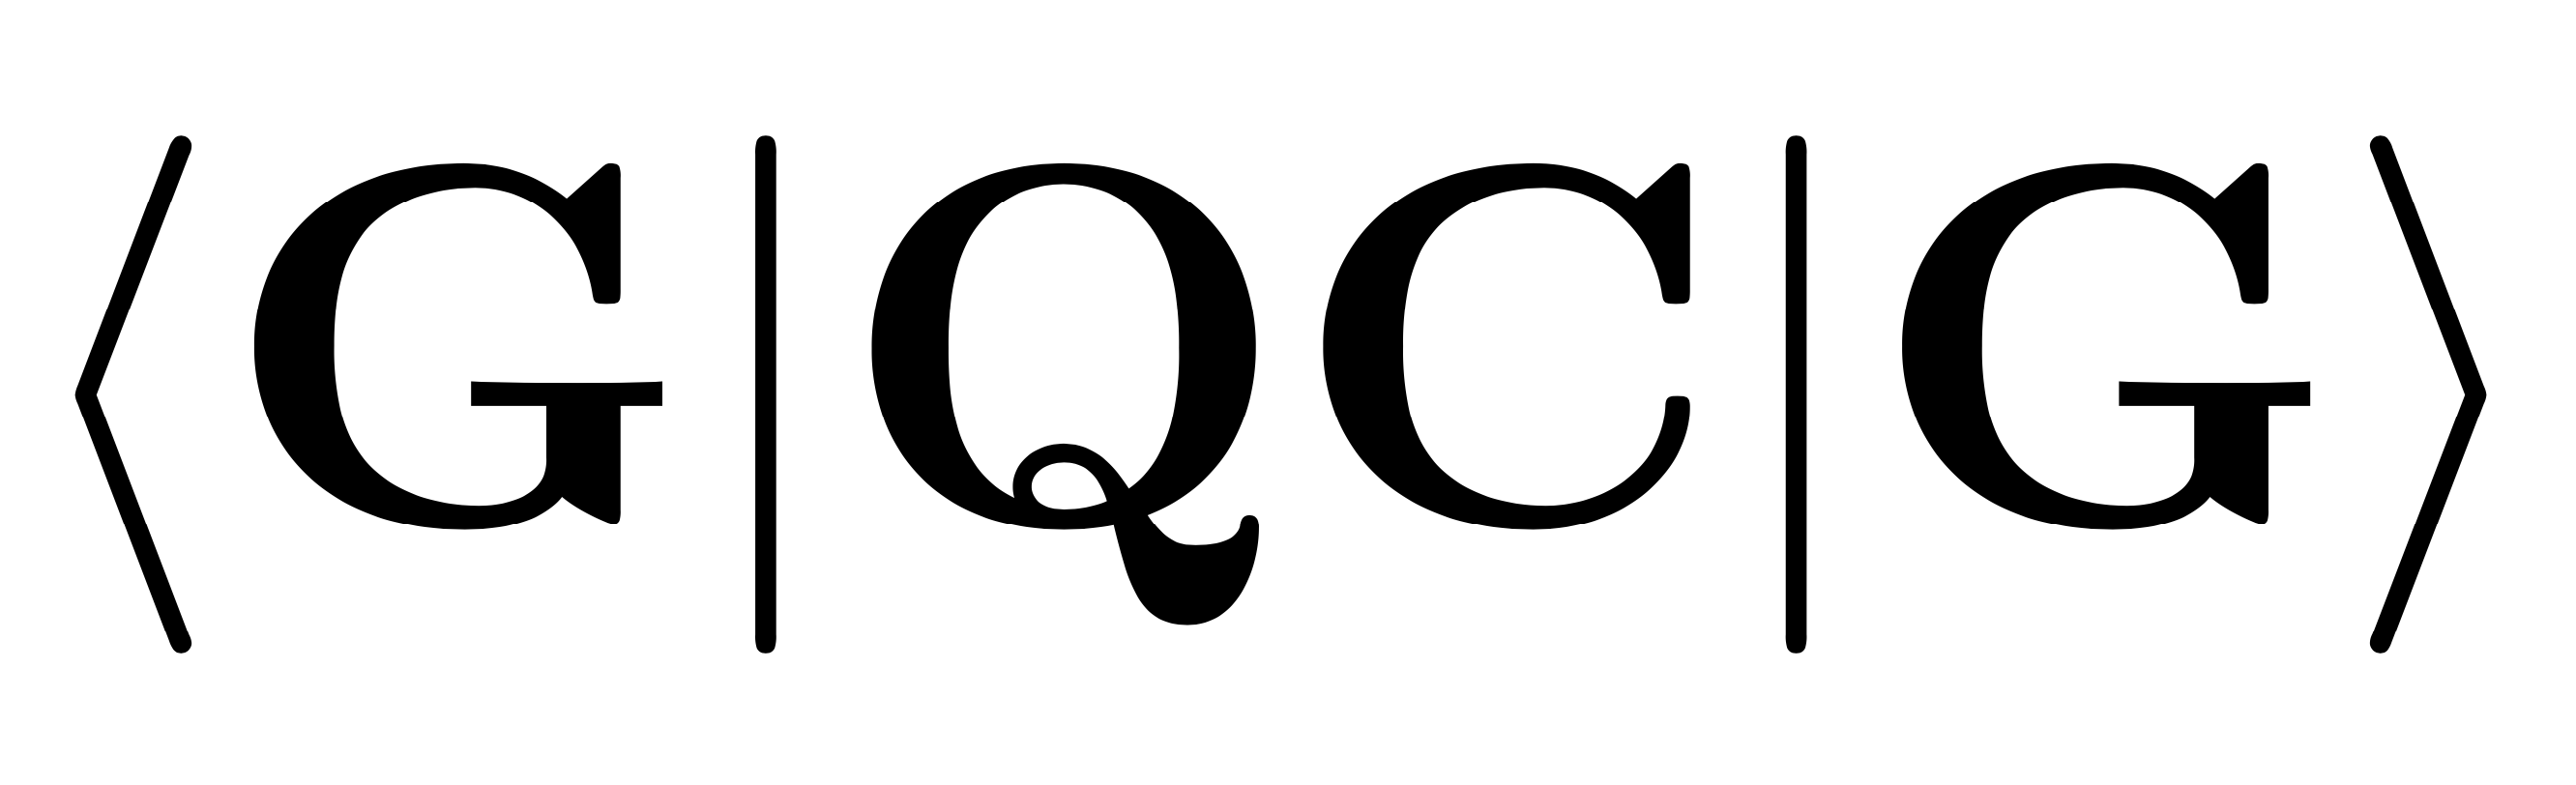
\includegraphics[height=3cm]{figures/gqcg_logo} & \includegraphics[height=3cm]{figures/fwo_logo}
        % \end{tabular}
        \begin{tabular}{l@{\hskip 1cm}c}
            \hspace{-1cm} 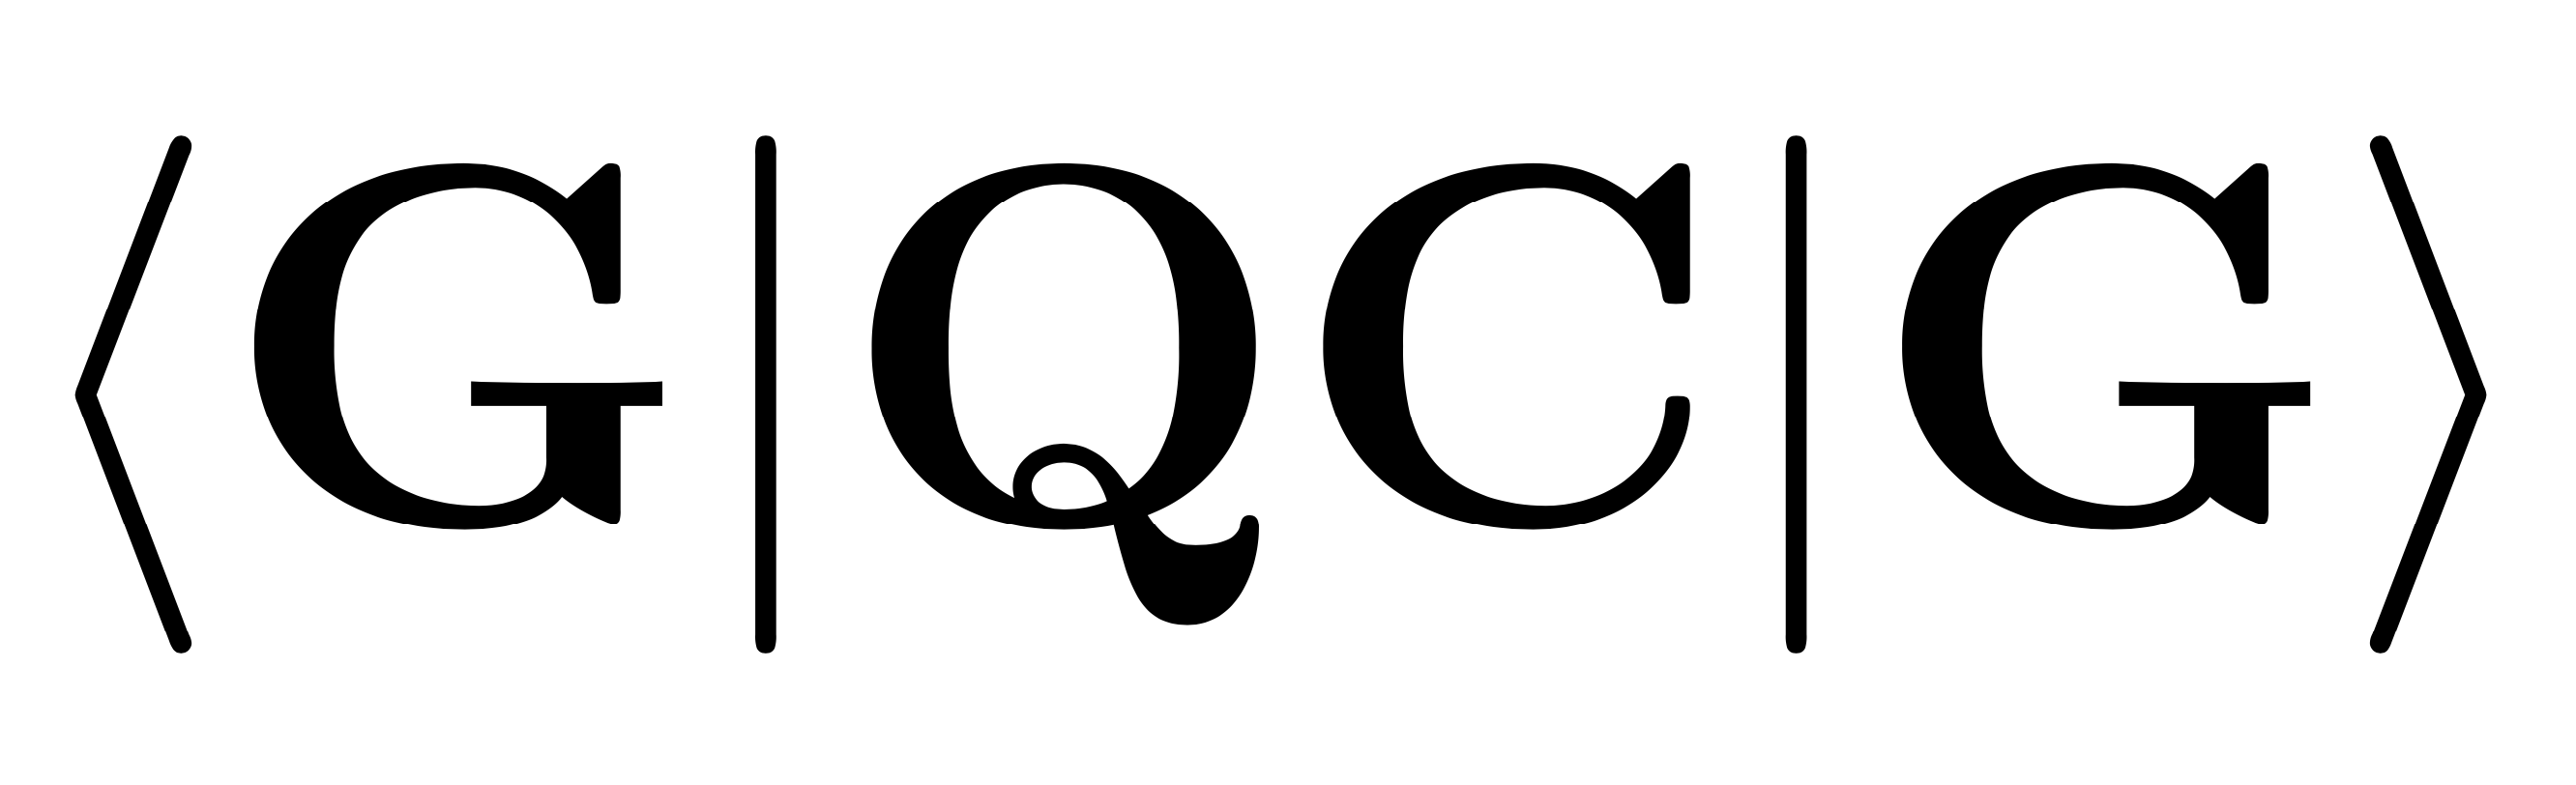
\includegraphics[height=3cm]{figures/gqcg_logo}
        \end{tabular}
    }


\end{columns}

\end{document}
